\documentclass[11pt]{article}

\usepackage[margin=1in]{geometry}
\usepackage{graphicx}
\usepackage{caption}
\usepackage{float}

\captionsetup{font=small, labelfont=bf, justification=raggedright,
              singlelinecheck=false}

% Overleaf: upload both figure PDFs anywhere in the project.
\graphicspath{{plots/}{./}}

\begin{document}

\section*{1. Figures and first patterns}

Figure~\ref{fig:china_links} reports, for each country and quarter, the share
of firms with an active Chinese supply-chain link. The source is FactSet
Revere. A firm counts if, at the close of the quarter, it has at least one
active relationship in which a Chinese company is either its customer or its
supplier; competitor links and looser partnership ties in the database are set
aside. The denominator is the set of firms in the same country with at least
one active customer or supplier relationship with any counterparty. I compute
the share within this supply-chain universe rather than over all companies in
the database, because Revere's firm coverage expands in large batches and
those batches would mechanically depress the ratio; a numerator and
denominator drawn from the same relationship data grow together, so the
coverage effect largely nets out. Quarters with fewer than fifty such firms
are not shown.

Figure~\ref{fig:us_holdings} tracks the growth of US institutional holdings
of European equity. The underlying series is the quarter-end market value of
every European stock held by US-domiciled institutional funds in FactSet
LionShares, including depositary receipts. FactSet reports these values in
dollars, converted at current exchange rates, which answers the currency
question: growth in the series mixes net purchases with valuation and
exchange-rate movements. I deflate by the US CPI, express everything in 2020
dollars, and plot year-over-year changes from 2005 onward; earlier years are
dominated by the database's own expansion. All panels share a common vertical
scale capped at $+200$ percent, so the few remaining coverage spikes run off
scale instead of compressing their panels.

Three patterns stand out so far.

\emph{Exposure is deepest in the continental manufacturing core, not in the
US or the UK.} Averaging over 2016--2024, the share of supply-chain-active
firms with a China link is 8.7 percent in Switzerland, 7.6--7.7 percent in
France, the Netherlands, and Germany, 5.7 percent in Italy, 5.5 percent in
the US, and about 4.3 percent in the UK.

\emph{The trade war did not visibly unwind these links.} The US share rises
from 5.2 percent in mid-2018 to 6.1 percent at end-2023; Germany goes from
6.4 to 8.9 percent, Switzerland from 6.8 to 10.4 percent over the same
window. Through the tariff rounds and the pandemic, the extensive margin of
China links kept widening. The first broad-based softening appears only in
2024 (US 6.1 to 5.4 percent, Germany 8.9 to 8.1). I cannot yet tell whether
that is genuine de-risking or simply Revere recording new relationships with
a lag, so I would not lean on it. The sharp drop in the very last quarter is
neither: the Revere universe jumps from about 34,000 to 51,000 US firms in
2025Q1, another coverage batch, and the ratio dilutes mechanically. The same
composition force explains why early-sample peaks (Germany at 25 percent in
2009) overstate exposure: the first firms covered in each country are its
largest multinationals, which are the most likely to trade with China.

\emph{For the dollar series, 2022 is the deepest real drawdown in the
sample.} Real holdings fall 42.8 percent year-over-year in 2022Q4, worse than
the trough of the financial crisis (39.7 percent in 2009Q1). Covid, by
contrast, barely registers: the worst quarter of 2020 is $-2.1$ percent. Part
of the 2022 collapse is the euro's depreciation, since the series is in
dollars. In levels, real holdings peak at \$2.2 trillion (2020 dollars) in
2021Q4 and stand at \$1.5 trillion at end-2023, still roughly 1.8 times the
pre-crisis peak of 2007.

\begin{figure}[p]
  \centering
  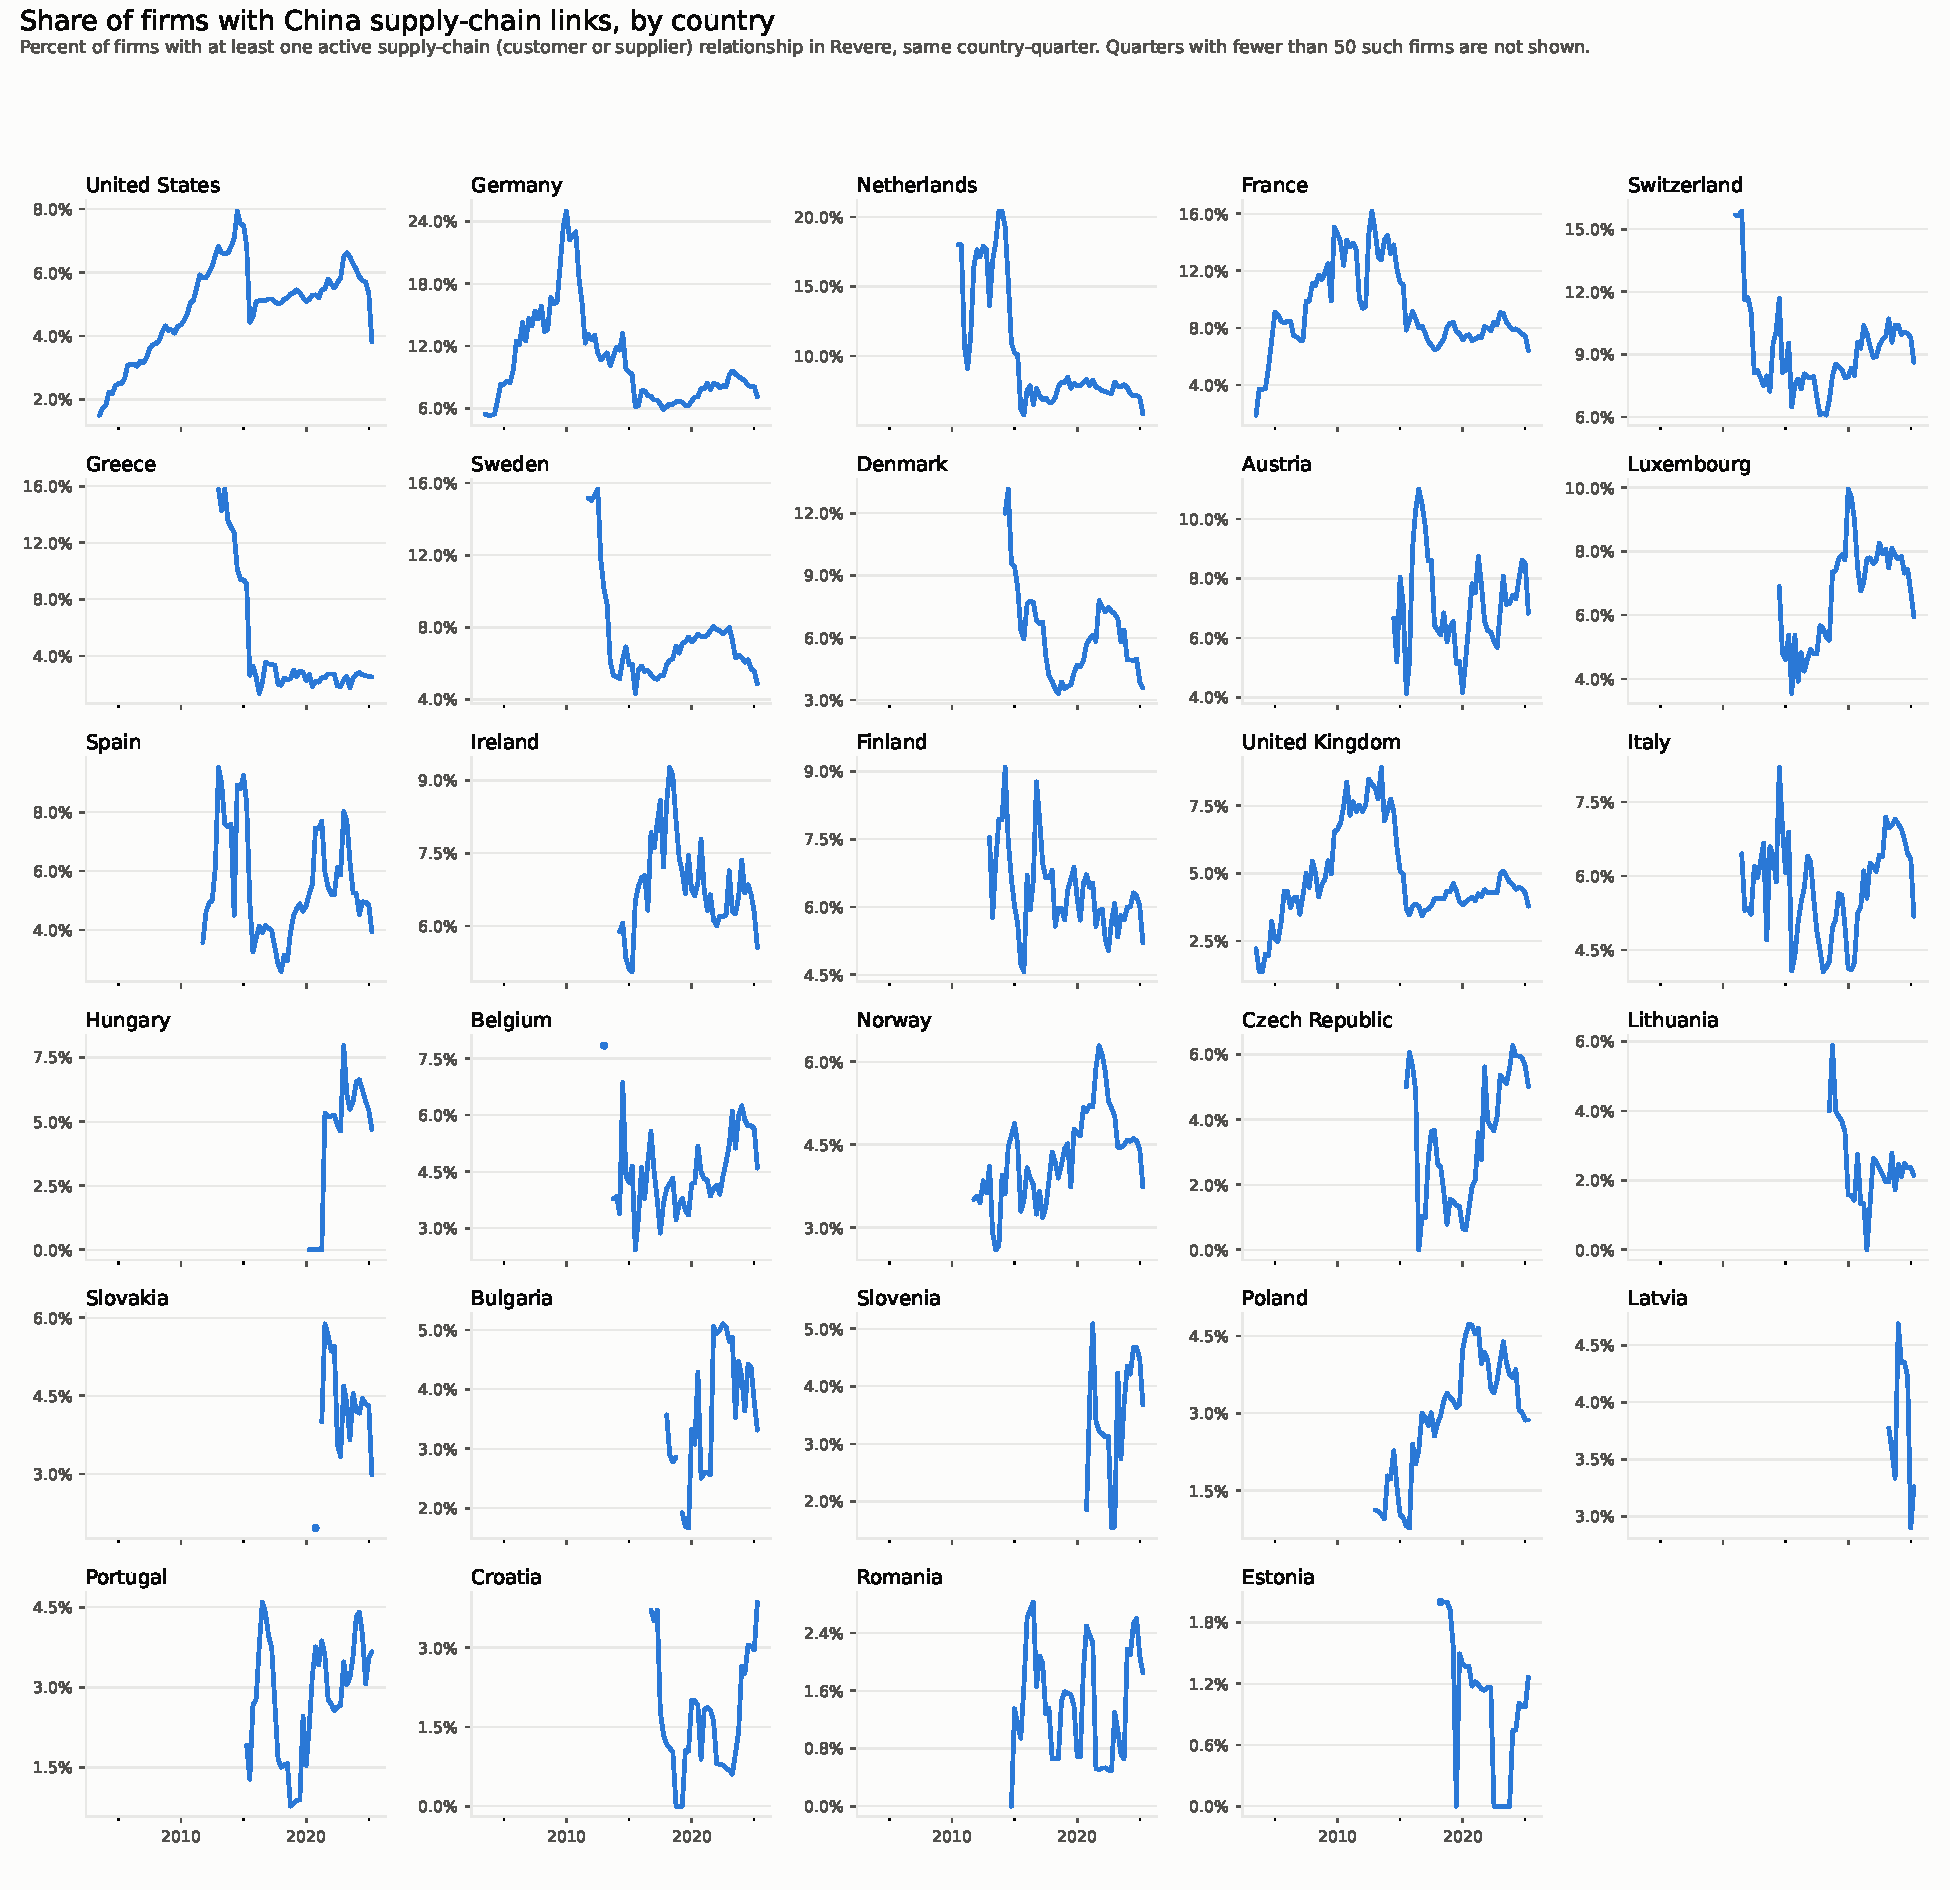
\includegraphics[width=\textwidth]{fig_china_link_fraction.pdf}
  \caption{Share of firms with an active Chinese supply-chain link, by
    country, 2003--2025. Each panel is one country; the vertical axis is the
    number of firms with at least one active customer or supplier
    relationship with a Chinese company, as a percent of firms with at least
    one active customer or supplier relationship with any counterparty in the
    same country-quarter. Quarters with fewer than fifty such firms are not
    shown.}
  \label{fig:china_links}
\end{figure}

\begin{figure}[p]
  \centering
  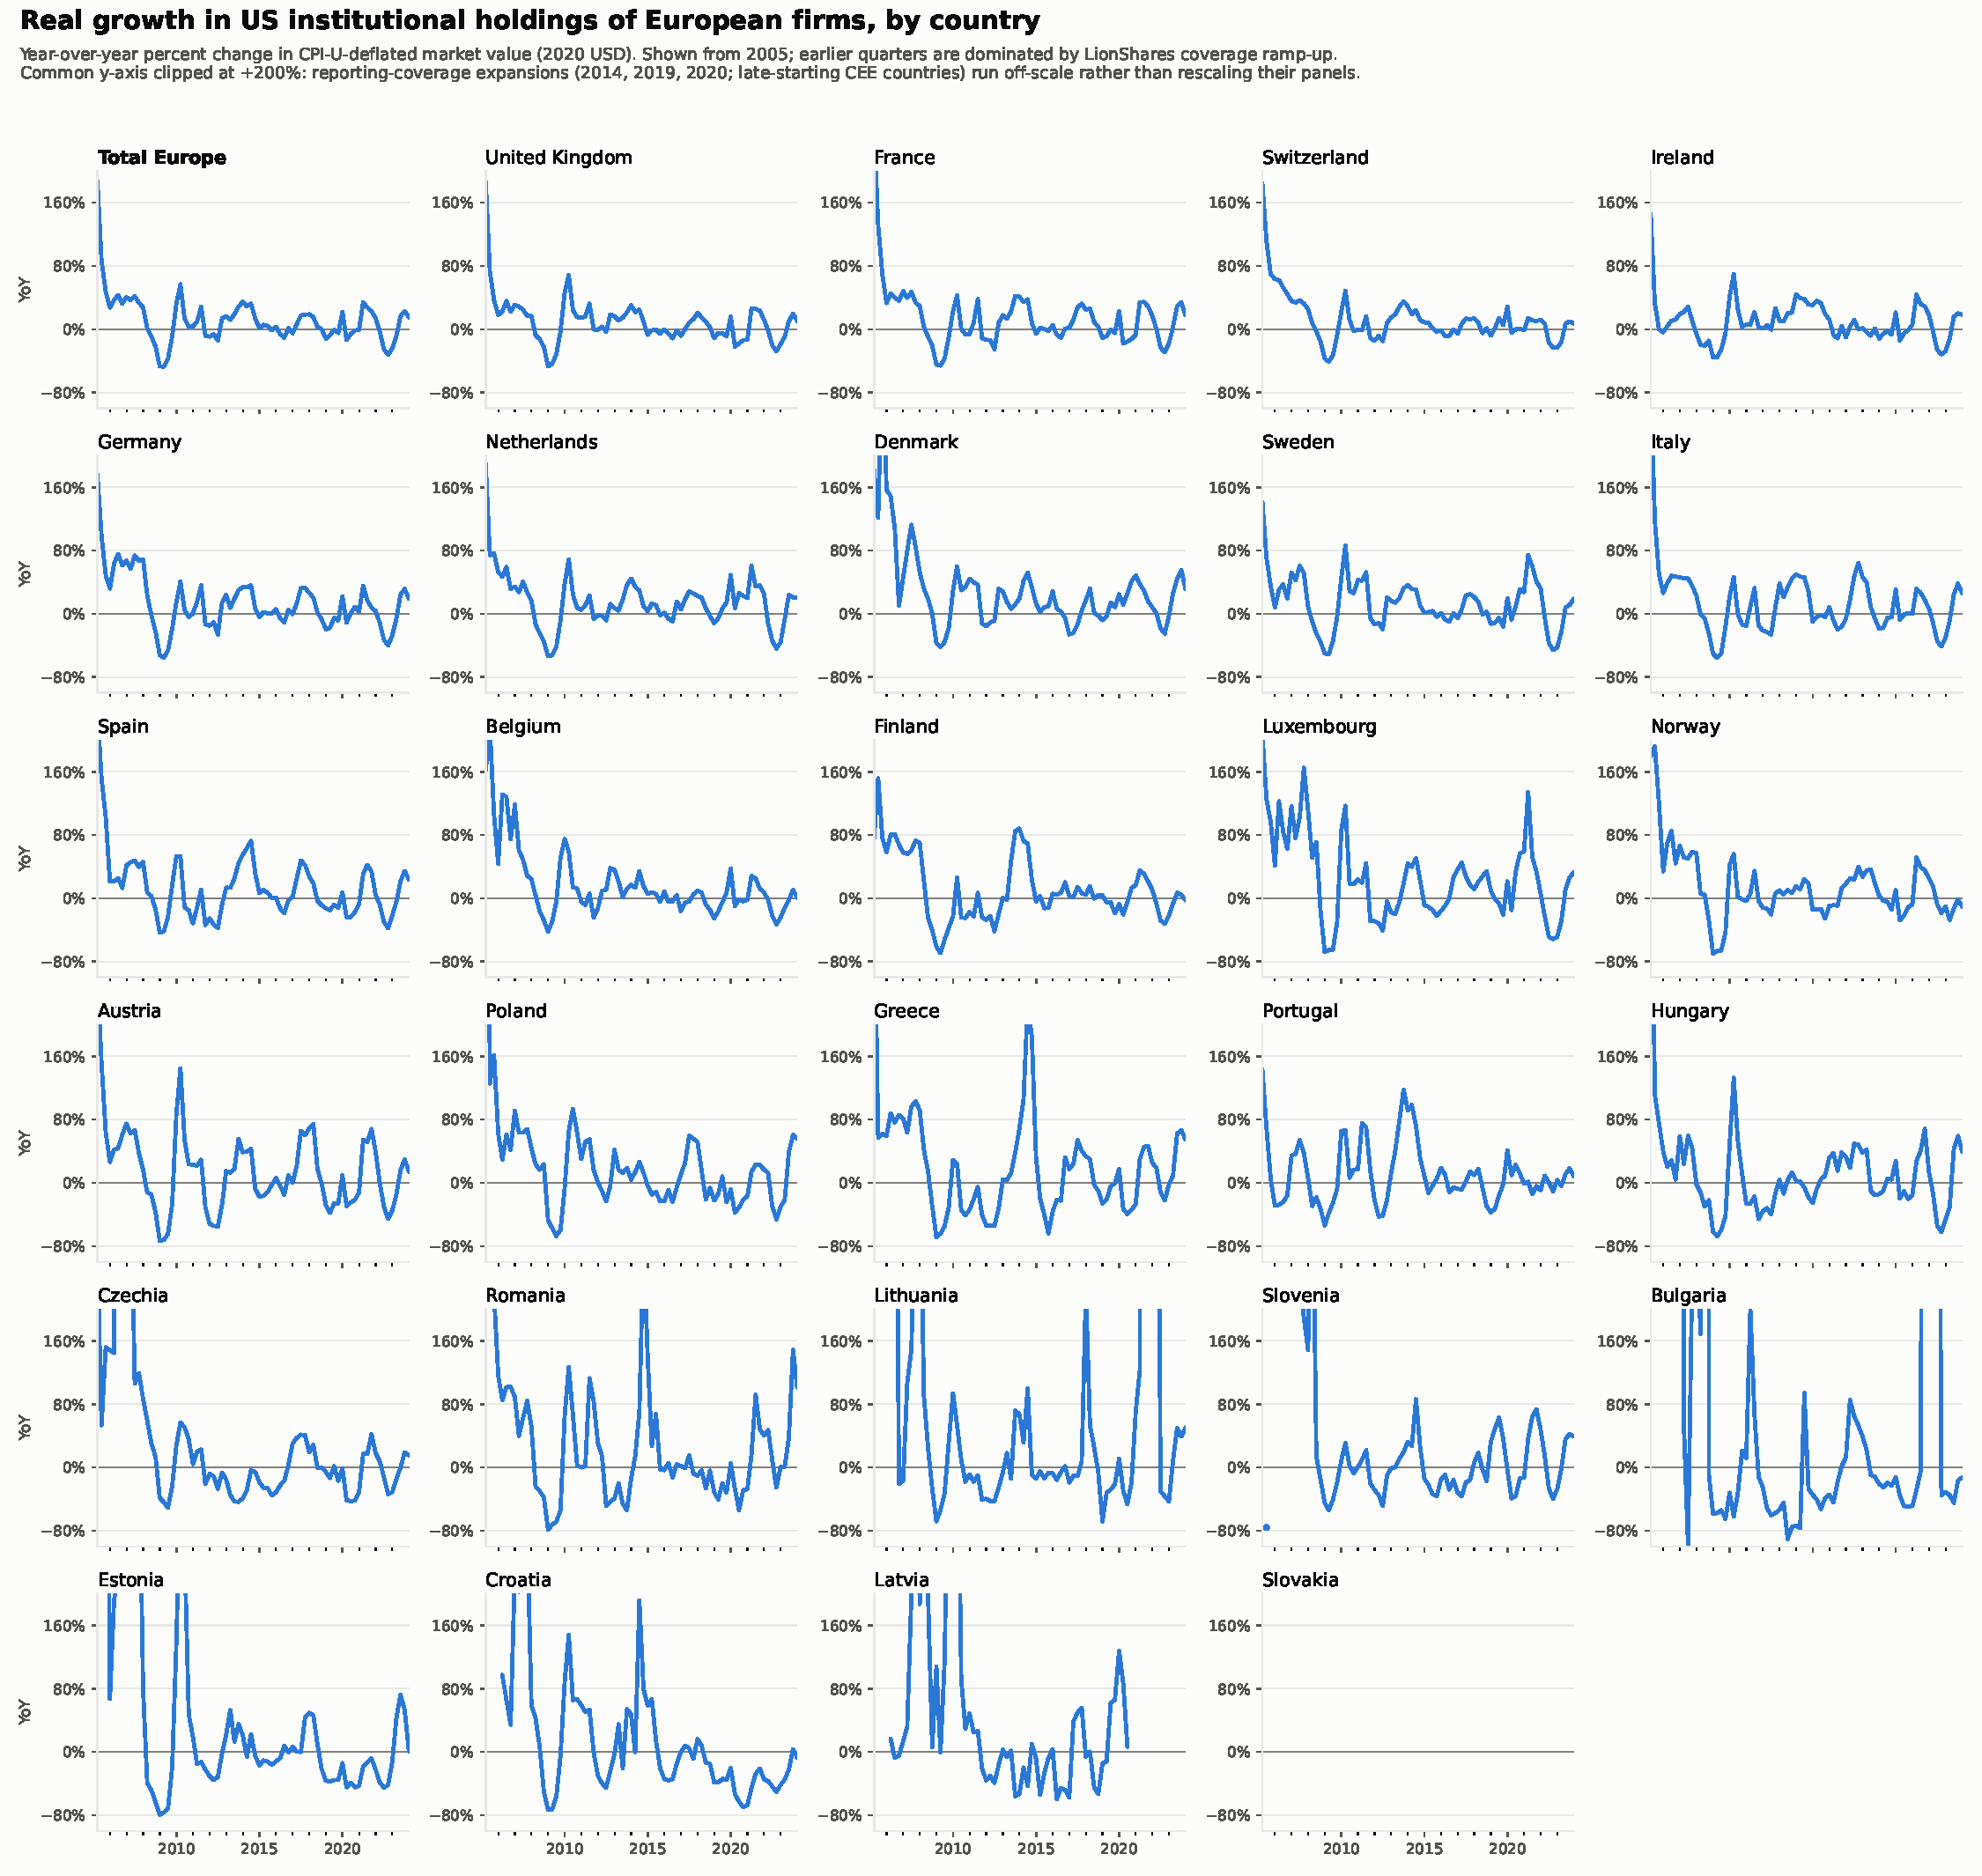
\includegraphics[width=\textwidth]{fig_us_holdings_real_yoy_growth.pdf}
  \caption{Real growth in US institutional holdings of European firms, by
    country, 2005--2023. Each panel is one country, and the first panel
    aggregates the 28-country European sample; the vertical axis is the
    year-over-year percent change in CPI-deflated market value (2020
    dollars) of equity held by US-domiciled institutional funds, on a common
    scale capped at $+200$ percent.}
  \label{fig:us_holdings}
\end{figure}

\section*{2. Beyond first-tier links: indirect China exposure}

A committee member raised a fair point: Revere records direct relationships,
so a firm whose own suppliers source from China carries hidden exposure that
my current measure misses. The production-network literature has a standard
answer. Let $W$ collect input shares, with $W_{ij}$ the share of firm $i$'s
purchases sourced from firm $j$ and rows summing to one, and let $1-\alpha$ be
the intermediate input share, the fraction of costs spent on inputs rather than
labor. Powers of the matrix trace successive tiers, direct suppliers then
suppliers of suppliers and so on, each tier discounted by a further factor of
$1-\alpha<1$, so the series converges. Its sum is the Leontief inverse
$[I-(1-\alpha)W']^{-1} = I + (1-\alpha)W' + (1-\alpha)^2 W'^2 + \dots$, which
accumulates a firm's reliance on any given source across every supply tier at
once (Acemoglu et al., 2012, Eq.~4). Dhyne et al. (2021) write the same object
at the firm level, as a fixed point in which a firm's total import share
equals its direct import share plus the input-share-weighted total shares of
its domestic suppliers.

\begin{thebibliography}{99}

\bibitem{acemoglu2012} Acemoglu, D., V. Carvalho, A. Ozdaglar, and
A. Tahbaz-Salehi (2012): ``The Network Origins of Aggregate Fluctuations,''
\emph{Econometrica}, 80(5), 1977--2016.

\bibitem{dhyne2021} Dhyne, E., A. K. Kikkawa, M. Mogstad, and F. Tintelnot
(2021): ``Trade and Domestic Production Networks,'' \emph{Review of Economic
Studies}, 88(2), 643--668.

\end{thebibliography}

\end{document}
